\chapter{Réseaux de neurones}

\section{Problème de classification}
Dans la théorie de l'apprentissage statistique, la classification a pour objectif de déduire d'un nombre fini d'observations indépendantes une partition de l'espace en un ensemble a priori inconnu de domaines de l'espace appelés classes. 

%%%%%%%%%%%%%%%%%%%%%%%%%%%%%%%%%%%%%%%%%%%%%%%%%%%%%%%%%%%%%%%%%%%%%%%%%%%%%%
%%% 		A compléter according to Muguette mais osef en vrai								%%%%
%%%%%%%%%%%%%%%%%%%%%%%%%%%%%%%%%%%%%%%%%%%%%%%%%%%%%%%%%%%%%%%%%%%%%%%%%%%%%%


\section{Apprentissage supervisé}

L'apprentissage supervisé est une branche de l'apprentissage automatique qui consiste à reproduire automatiquement des règles à partir d'une base de données d'apprentissage labellisée.
A partir de ces exemples, on apprend donc à reconnaitre chaque élément et à le labelliser correctement. L'objectif final est alors de pouvoir généraliser cet apprentissage.
Ainsi, si l'on prend l'exemple (que l'on appliquera plus tard avec MNIST) d'une base de données de chiffres manuscrits, on apprend à reconnaitre les chiffres parmi cette base, en espérant pouvoir obtenir une généralisation qui nous permettra de reconnaitre par la suite n'importe quel chiffre manuscrit.

On peut distinguer l'apprentissage supervisé de l'apprentissage non-supervisé, qui lui consiste à créer des règles à partir d'une base de données fournie, qui n'aura alors pas de labels pré-définis. Le système devra alors trouver des patterns, des caractéristiques communes entre les éléments pour les regrouper en de nouveaux labels.

\section{Structure d'un neurone}

L'extraordinaire capacité d'apprentissage et d'adaptation des réseaux de neurones biologiques a poussé les scientifiques à tenter de modéliser informatiquement leur fonctionnement afin d'exploiter ces capacités. 

Les observations biologiques ont mené au premier modèle du neurone, divisé en 3 parties. Le neurone reçoit des signaux chimio-électriques par ses dendrites; ces signaux sont traités dans le corps cellulaire, où un effet de seuil est appliqué; enfin l'axone permet la transmission du signal chimio-électrique de sortie. De nouvelles découvertes sur les neurones ont permis de complexifier grandement ce modèle, mais c'est celui qui sert de base aux neurones artificiels. \\

\begin{definition}[Neurone] 
Un neurone à $n$ entrées permet de modéliser une fonction de $\R^n$ dans $\R$. Un neurone est défini par la données de trois paramètres :
  \begin{itemize}
    \item un vecteur de poids $\omega \in \R^n$
    \item un biais $b \in \R$
    \item une fonction d'activation $g \in \R^\R$
  \end{itemize}

La fonction $f$ modélisée par le neurone s'écrit alors : 
  \begin{equation}
\forall x \in \R^n, f(x) = g(\omega^{T}x - b) = g(\sum_{i=0}^{n-1}\omega_{i}x_{i} - b)
  \label{neuron_function_equation}
  \end{equation}
\end{definition}    
\begin{remark}[Biais]
Il est possible de rajouter une composante $x_{n} = -1$ à tous les vecteurs d'entrées afin de pouvoir considérer le biais $b$ comme la composante $\omega_n$ du vecteur de poids. L'équation \eqref{neuron_function_equation} devient alors
  \begin{equation}
\forall x \in \R^n, f(x) = g(\omega^{T}x) = g(\sum_{i=0}^{n}\omega_{i}x_{i})  
  \label{corrected_neuron_function_equation}
  \end{equation}

Cependant, considérer le biais comme un poids pose des problèmes lorsqu'on utilise l'approche des graphes de calculs, qui sera explicitée dans la suite de ce rapport. Nous n'avons donc pas appliqué cette simplification pour nos propres réseaux.

\end{remark}

\section{Réseaux de neurones}

Un neurone permet, en prenant n entrées, de renvoyer en sortie une valeur réelle entre 0 (ou -1) et 1. Au vu des fonctions d'activation utilisées, les réponses renvoyées peuvent être assimilées à des booléens (0 : 1). La fonction de transfert du réseau de neurone étant une combinaison linéaire à qui on applique le créneau (fonction d'activation), un neurone seul peut séparer un plan en deux. 
Par exemple, en prenant un réseau à deux entrées, une sortie, dans un problème de classification classique, ce réseau permet de séparer le plan (x,y) en deux parties séparées par une droite, comme montré ci-dessous :

\begin{figure}[h]
\begin{center}
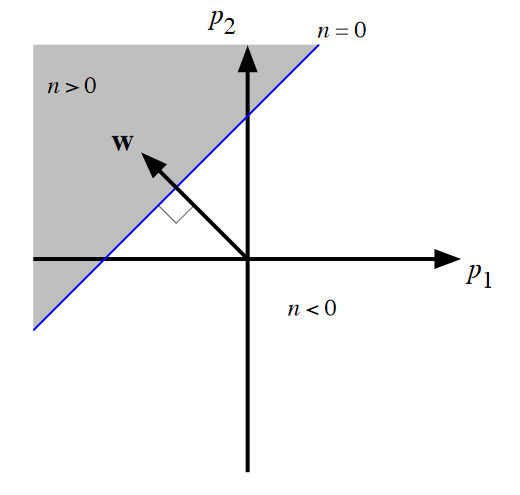
\includegraphics[width=0.5\textwidth]{images/decisionNeuroneSeul.png}\caption{Classification pour un neurone seul à deux entrées, une sortie}
\end{center}
\end{figure} 

Un neurone seul ne peut donc que séparer un plan en deux parties. Les possibilités limitées d'un neurone seul ont donc poussé l'informatique à agencer les neurones en réseaux afin de créer des modèles plus complexes. Ainsi, un réseau à deux couches peut (à condition d'avoir suffisamment de neurones dans ces couches) identifier tout zone convexe d'un espace vectoriel, alors qu'un réseau à 3 couches peut séparer toute partie de cet espace. On agence alors les neurones en réseaux afin de créer des modèles plus complexes. \\

\begin{definition}[Réseau de neurone - Perceptrons] 
Un réseau de neurones est défini par un graphe orienté $\mathcal{G}(V, A)$ où les n\oe{}uds sont des neurones, les arêtes des liens entre les neurones et par un ensemble de neurones d'entrée $V_{in} \subset V$ et de neurones de sorties $V_{out} \subset V$. Une arête partant d'un neurone $i$ vers un neurone $j$ signifie que la sortie du neurone $i$ est une entrée pour le neurone $j$. Notons $f_{j}$ la fonction représentant le neurone $j$. Finalement, nous noterons un réseau $\mathcal{N}(V, A, V_{in}, V_{out}, f)$ où $f$ est l'ensemble des fonctions des neurones.\\
\end{definition}

\begin{definition}[Perceptron]
Un réseau de neurones est de type perceptron lorsque le graphe qui le représente est acyclique (réseau feedforward) et qu'il peut être représenté comme une suite finie de couches de neurones telle que les sorties d'une couche sont exactement les entrées de la couche suivante.
\end{definition} 

\section{Propagation dans un perceptron}

On cherche à obtenir les équations qui régissent la propagation des entrées dans un réseau perceptron. Comme les neurones sont agencées par couches, on peut indicer chaque neurone par son numéro de couche et sa position dans la couche. De plus, on parlera dans la suite indistinctement du neurone ou de la fonction qu'il modélise. 

Alors, soit un réseau perceptron à $N$ couches. Pour $i \in \brackets{1,\ N}$ soit $n_i$ le nombre de neurones de la couche $i$. Pour tout $i,j $ tel que $i \in \brackets{1,\ N}, j \in \brackets{1,\ n_i}$, le neurone $(i,j)$ est défini par 
\begin{itemize}
  \item sa fonction d'activation $f_{i,j}$ 
  \item son vecteur de poids $\omega_{i,j}$
  \item son biais $b_{i,j}$
\end{itemize}

Comme on est dans un réseau perceptron, tous les neurones de la couche $i-1$ sont connectés au neurone $(i,j)$. Par conséquent le vecteur d'entrée de ce neurone est un vecteur $X_n$ de dimension $n_{i-1} \times 1$. Alors la sortie du neurone $(i,j)$ est égale à $f_{i,j}(\omega_{i,j}X_{i-1}^T - b_{i,j})$. En écrivant $X_n = \begin{pmatrix}X_0^n & ... & X_{n_i-1}^n\end{pmatrix}^T$, on a alors la relation de récurrence 
\begin{equation}
  X_i^{j+1} = f_{j,i}(\omega_{j,i}X_j^T - b_{j,i})
  \label{equation_propagation_coefficients}
\end{equation}

Dans un réseau perceptron, on suppose de plus que toutes les fonctions d'activations des neurones d'une même couche sont identiques. On a alors $\forall i \in \brackets{1,\ N},\ \forall j \in \brackets{1,\ n_i},\ f_{i,j} = f_i$
On peut alors réécrire l'équation \eqref{equation_propagation_coefficients} sous forme matricielle. On pose

\begin{align*}
\forall i \in \brackets{1,\ N},\ F_i &= \begin{pmatrix} f_i & ... & f_i \end{pmatrix}\quad \text{(Fonction d'activation de la couche)}\\
                            W_i &= \begin{pmatrix} \omega_{i,0} \mid & ... & \mid \omega_{i, n_i-1}\end{pmatrix}^T \quad \text{(Matrice des poids de la couche)} \\
                            B_i &= \begin{pmatrix} b_{i, n_i-1} & ... & b_{i, n_i-1}\end{pmatrix}^T 
\end{align*}

En nommant $X_0$ le vecteur en entrée du perceptron, on a la nouvelle équation matricielle : 
\begin{equation}
  \forall i \in \brackets{1,\ N},\ X_i = F_i(W_i X_{i-1} - B_i) 
  \label{equation_propagation_matricielle}
\end{equation}

\section{Rétropropagation}
%%%%%%%%%%%%%%
% OMG on n'avait pas de partie dessus ? :o 
%%%%%%%%%%%%%%
On a dans toutes nos implémentations pris un pas de rétropropagation de $dx=0,01$.